\documentclass[conference]{IEEEtran}
\IEEEoverridecommandlockouts
% The preceding line is only needed to identify funding in the first footnote. If that is unneeded, please comment it out.
\usepackage{cite}
\usepackage{amsmath,amssymb,amsfonts}
\usepackage{algorithmic}
\usepackage{graphicx}
\usepackage{textcomp}
\usepackage{xcolor}
\usepackage{subfig}
\usepackage{multirow}
\usepackage{booktabs}

\def\BibTeX{{\rm B\kern-.05em{\sc i\kern-.025em b}\kern-.08em
    T\kern-.1667em\lower.7ex\hbox{E}\kern-.125emX}}
    
\usepackage[nomain, toc, acronym]{glossaries}
\glsdisablehyper

\newcommand\note[2]{{\color{#1}#2}}
\newcommand\todo[1]{{\note{red}{TODO: #1}}}

\newcommand{\unsw}{UNSW-NB15}
\newcommand{\cic}{CIC-IDS-2017}

\newacronym{dl}{DL}{Deep Learning}
\newacronym{ad}{AD}{Anomaly Detection}
\newacronym{ml}{ML}{Machine Learning}
\newacronym{ttl}{TTL}{Time-to-Live}
\newacronym{ids}{IDS}{Intrusion Detection System}
\newacronym{mlp}{MLP}{Multilayer Perceptron}
\newacronym{relu}{ReLU}{Rectified Linear Unit}
\newacronym{ip}{IP}{Internet Protocol}

\begin{document}

\title{EagerNet: Early Intrusion Prediction\\in Feed Forward Neural Networks}

\author{\IEEEauthorblockN{Fares Meghdouri, Maximilian Bachl and Tanja Zseby}
\IEEEauthorblockA{Technische Universität Wien\\
Vienna, Austria\\
firstname.lastname@tuwien.ac.at}}



\maketitle

\begin{abstract}

\end{abstract}

\begin{IEEEkeywords}

\end{IEEEkeywords}

\section{Introduction}

\section{Supervised Learning for Network Intrusion Detection}

\section{Eager-Stopping}
\subsection{Feed Forward Neural Networks}

\subsection{Early Predictions}
\subsubsection{Combined Back-propagation Loss}

\begin{equation}
l = \frac{1}{N} \sum_{n}^{N} -\omega [y_n \cdot \log \sigma (x_{n}) + (1 - y_n) \cdot \log (1 - \sigma (x_{n}))]
\end{equation}

\[
\nabla l = \underbrace{W_{current} \times \nabla l_{current}}_{\text{Current gradient}} + \underbrace{\sum_{i}^{} \nabla l_{i}}_{\text{Next layer gradients}}
\]

\begin{figure*}[htp]
\center
\subfloat[Conventional Feed Forward Neural Network.]{%
  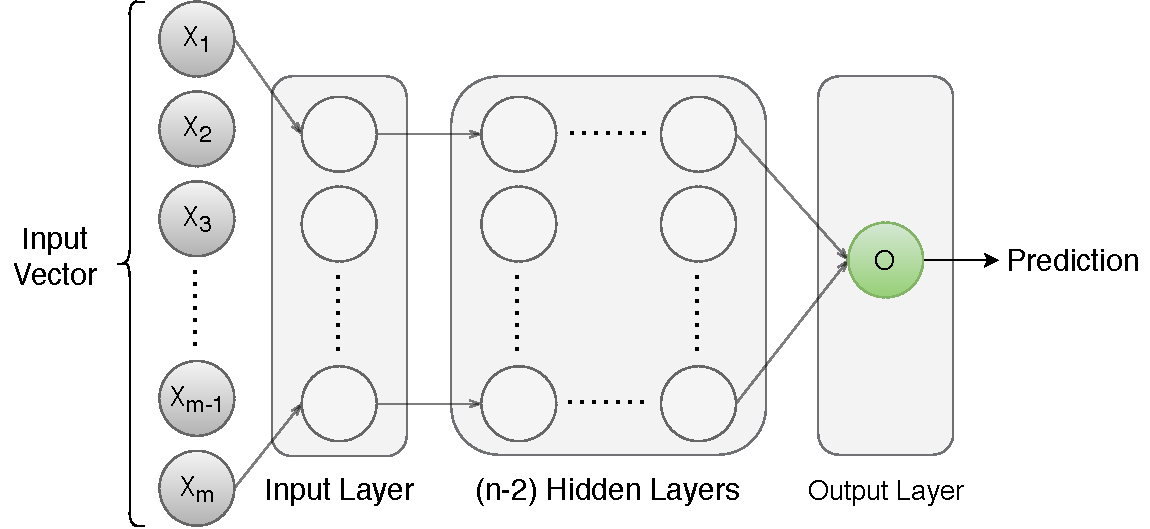
\includegraphics[clip,width=0.45\textwidth]{figures/ffnn_new.pdf}%
}
\\
\subfloat[Eager-Stopping Neural Network: forward-propagation mode.]{%
  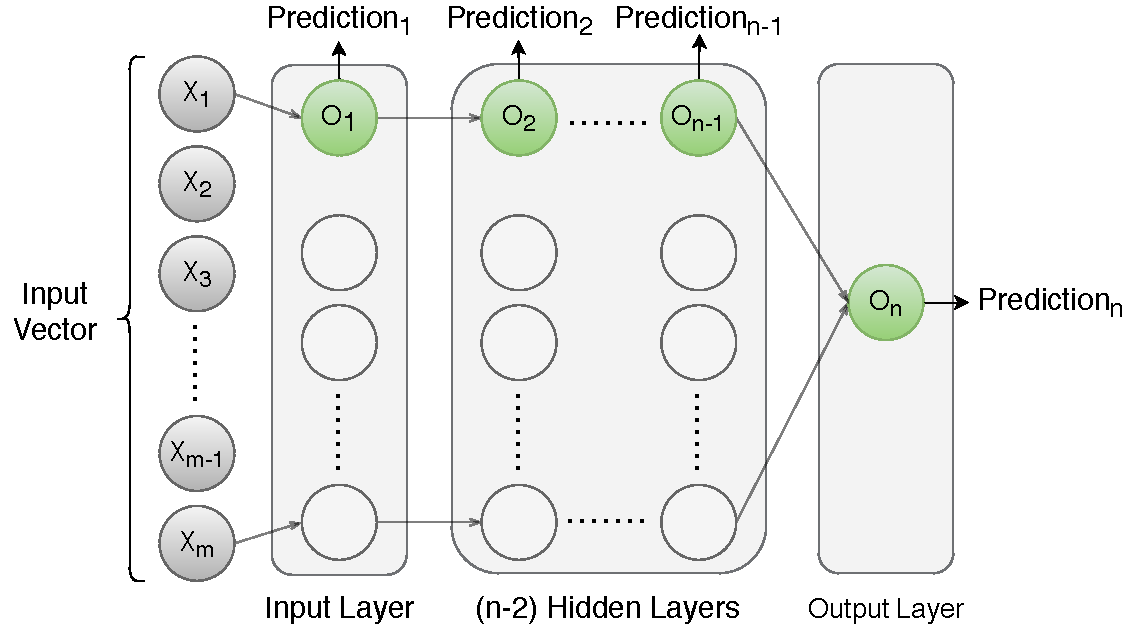
\includegraphics[clip,width=0.53\textwidth]{figures/eagernet_new.pdf}%
}
\quad
\subfloat[Eager-Stopping Neural Network: back-propagation mode.]{%
  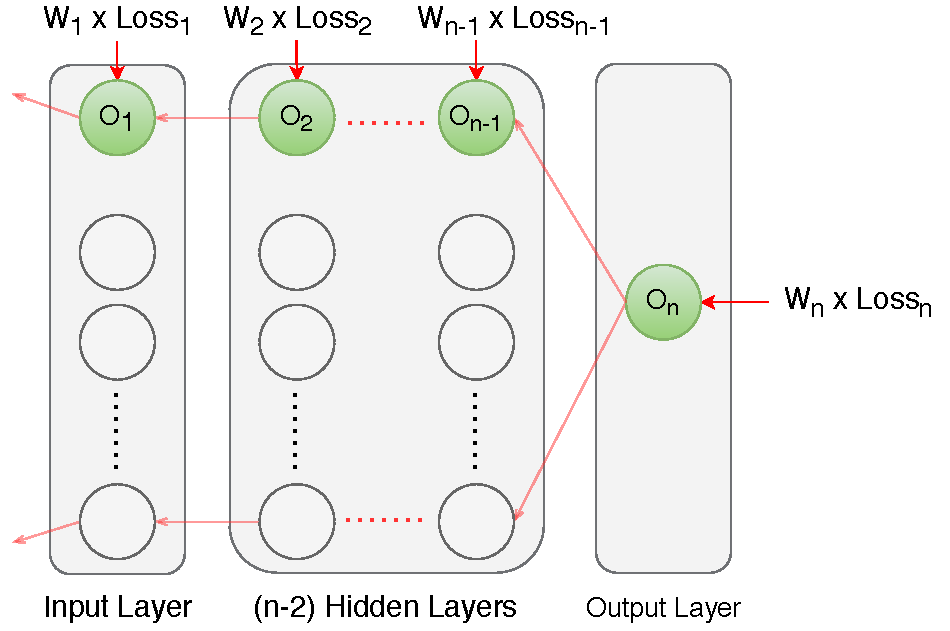
\includegraphics[clip,width=0.45\textwidth]{figures/eagernet_backprop_new.pdf}%
}

\caption{The difference between conventional neural networks and our proposed architecture.}

\end{figure*}


\section{Related Work}

\section{Evaluation and Discussion}
\subsection{Datasets}

\begin{table}[ht!]
	
	\centering
	\caption{CAIA Flow Features.}
	\label{tab:cres}
	     
	\footnotesize
	\begin{tabular}{|c|c|c|}
		\toprule
		\textbf{Direction}                    & \textbf{Features}        & \textbf{Statistical Operations}        \\
		\midrule
		    
		                                      & flowDurationMilliseconds &                                        \\
		                                      & sourceTransportPort      &                                        \\
		                                      & destinationTransportPort &                                        \\
		                                      & protocolIdentifier       &                                        \\
		                                      & octetTotalCount          &                                        \\
		\midrule
		\multirow{7}{*}{Forward and Backward} & ipTotalLength            & \multirow{2}{*}{Mean, Min, Max, Stdev} \\
		                                      & interPacketTimeSeconds   &                                        \\
		\cmidrule{2-3}
		                                      & packetTotalCount         &                                        \\
		                                      & tcpSynTotalCount         &                                        \\
		                                      & tcpAckTotalCount         &                                        \\
		                                      & tcpFinTotalCount         &                                        \\
		                                      & tcpCwrTotalCount         &                                        \\
		   
		\midrule
		
		
	\end{tabular}
		
\end{table}

\subsection{Binary vs. Multiclass Classification}

\begin{table*}
\parbox{.45\linewidth}{
\centering
\begin{tabular}{cccrrrr}
\toprule
\textbf{Variant} & \textbf{Weights} & \textbf{Layers} & \textbf{Acc.} & \textbf{Prec.} & \textbf{Rec.} & \textbf{J.}\\
\midrule
\multirow{6}{*}{\rotatebox{90}{Binary}} & \multirow{2}{*}{Equal} & 1-3-1 & & & & \\
 & & 1-1-1 & & & & \\
 & \multirow{2}{*}{Increasing} & 1-3-1 & & & & \\
 & & 1-1-1 & & & & \\
 & \multirow{2}{*}{Decreasing} & 1-3-1 & & & & \\
 & & 1-1-1 & & & & \\
\midrule
\multirow{6}{*}{\rotatebox{90}{Multiclass}} & \multirow{2}{*}{Equal} & 1-3-1 & & & & \\
 & & 1-1-1 & & & & \\
 & \multirow{2}{*}{Increasing} & 1-3-1 & & & & \\
 & & 1-1-1 & & & & \\
 & \multirow{2}{*}{Decreasing} & 1-3-1 & & & & \\
 & & 1-1-1 & & & & \\
\end{tabular}
\caption{CIC-IDS17}
}
\hfill
\parbox{.45\linewidth}{
\centering
\begin{tabular}{cccrrrr}
\toprule
\textbf{Variant} & \textbf{Weights} & \textbf{Layers} & \textbf{Acc.} & \textbf{Prec.} & \textbf{Rec.} & \textbf{J.}\\
\midrule
\multirow{6}{*}{\rotatebox{90}{Binary}} & \multirow{2}{*}{Equal} & 1-3-1 & & & & \\
 & & 1-1-1 & & & & \\
 & \multirow{2}{*}{Increasing} & 1-3-1 & & & & \\
 & & 1-1-1 & & & & \\
 & \multirow{2}{*}{Decreasing} & 1-3-1 & & & & \\
 & & 1-1-1 & & & & \\
\midrule
\multirow{6}{*}{\rotatebox{90}{Multiclass}} & \multirow{2}{*}{Equal} & 1-3-1 & & & & \\
 & & 1-1-1 & & & & \\
 & \multirow{2}{*}{Increasing} & 1-3-1 & & & & \\
 & & 1-1-1 & & & & \\
 & \multirow{2}{*}{Decreasing} & 1-3-1 & & & & \\
 & & 1-1-1 & & & & \\
\end{tabular}
\caption{UNSW-NB15}
}
\end{table*}



\begin{table}

\centering
\begin{tabular}{ccrr}
\toprule
\textbf{Dataset} & \textbf{Architecture} & \textbf{FFNN} & \textbf{EagerNet*}\\
\midrule
\multirow{6}{*}{\rotatebox{90}{CIC-IDS17}} & & & \\
 & & & \\
 & & & \\
 & & & \\
 & & & \\
 & & & \\
\midrule
\multirow{6}{*}{\rotatebox{90}{UNSW-NB15}} & & & \\
 & & & \\
 & & & \\
 & & & \\
 & & & \\
 & & & \\
\midrule
\multirow{6}{*}{\rotatebox{90}{MNIST}} & & & \\
 & & & \\
 & & & \\
 & & & \\
 & & & \\
 & & & \\
\end{tabular}
\vspace{1ex}

{\raggedright * . \par}
\caption{Accuracy scores.}


\end{table}

\begin{figure}[b!]
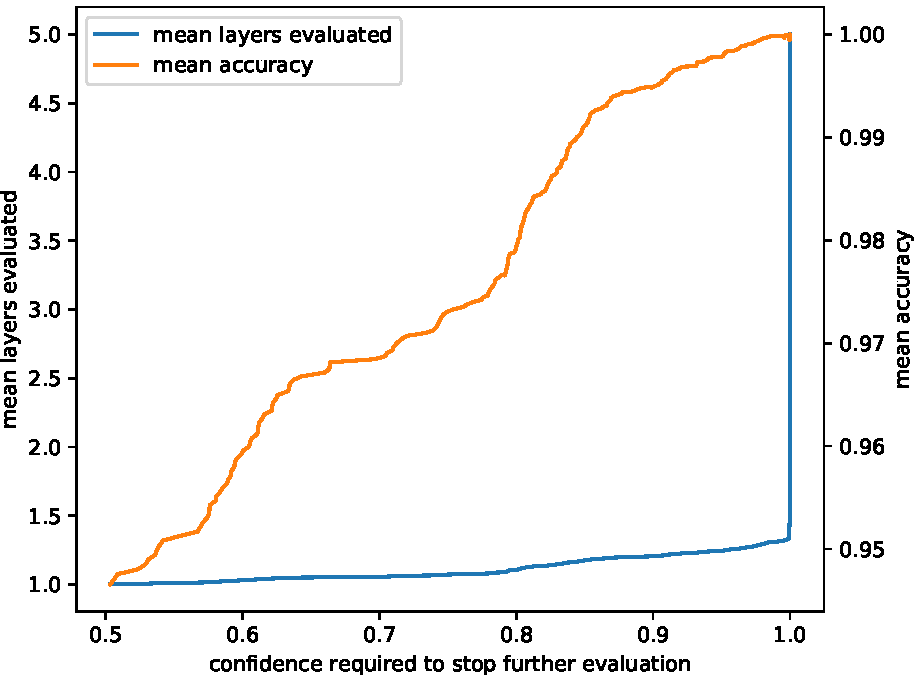
\includegraphics[width=\columnwidth]{figures/conf_acc_Jul10_15-09-38_gpu_0_3.pdf}
\caption{Accuracy-Confidence plot.\note{red}{FM: this will change}}
\label{fig:pdp_ttl}
\end{figure}

\begin{figure}[b!]
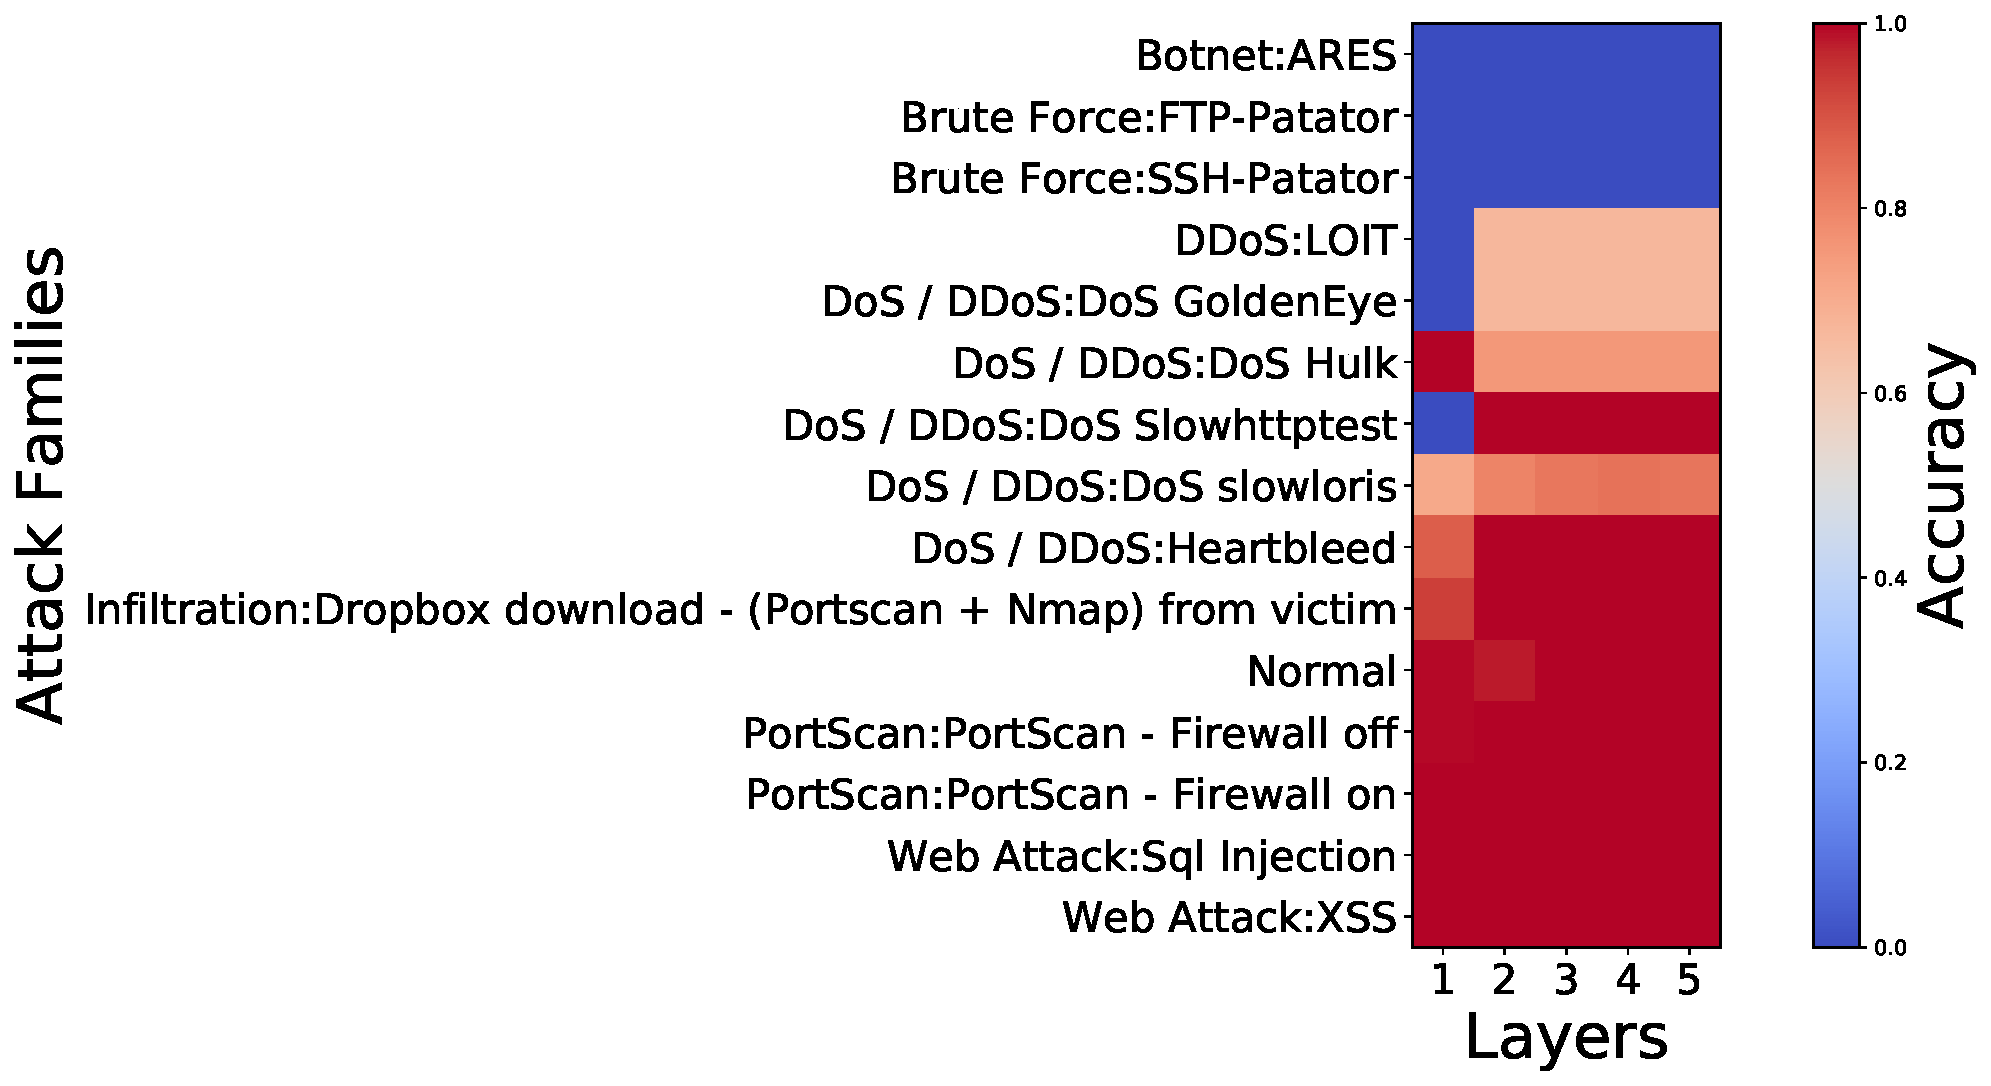
\includegraphics[width=\columnwidth]{figures/acc_multiclass_Jul10_15-18-24_gpu_0_3.pdf}
\caption{Accuracy plot multiclass.\note{red}{FM: this will change}}
\label{fig:pdp_ttl}
\end{figure}


\section{Conclusion}


\section*{Acknowledgements}
The Titan Xp used for this research was donated by the NVIDIA Corporation.

\bibliographystyle{ACM-Reference-Format}
\bibliography{bibliography}

\end{document}
